%%%%%%%%%%%%%%%%%%%%%%%%%%%%%%%%%%%%%%%%%
% Beamer Presentation
% LaTeX Template
% Version 1.0 (10/11/12)
%
% This template has been downloaded from:
% http://www.LaTeXTemplates.com
%
% License:
% CC BY-NC-SA 3.0 (http://creativecommons.org/licenses/by-nc-sa/3.0/)
%
%%%%%%%%%%%%%%%%%%%%%%%%%%%%%%%%%%%%%%%%%

%----------------------------------------------------------------------------------------
%	PACKAGES AND THEMES
%----------------------------------------------------------------------------------------

\documentclass[slidestop,compress,11pt,xcolor=dvipsnames]{beamer}

\mode<presentation> {

% The Beamer class comes with a number of default slide themes
% which change the colors and layouts of slides. Below this is a list
% of all the themes, uncomment each in turn to see what they look like.

%\usetheme{default}
%\usetheme{AnnArbor}
%\usetheme{Antibes}
%\usetheme{Bergen}
%\usetheme{Berkeley}
%\usetheme{Berlin}
%\usetheme{Boadilla}
%\usetheme{CambridgeUS}
%\usetheme{Copenhagen}
%\usetheme{Darmstadt}
%\usetheme{Dresden}
%\usetheme{Frankfurt}
%\usetheme{Goettingen}
%\usetheme{Hannover}
%\usetheme{Ilmenau}
%\usetheme{JuanLesPins}
%\usetheme{Luebeck}
\usetheme{Madrid}
%\usetheme{Malmoe}
%\usetheme{Marburg}
%\usetheme{Montpellier}
%\usetheme{PaloAlto}
%\usetheme{Pittsburgh}
%\usetheme{Rochester}
%\usetheme{Singapore}
%\usetheme{Szeged}
%\usetheme{Warsaw}

% As well as themes, the Beamer class has a number of color themes
% for any slide theme. Uncomment each of these in turn to see how it
% changes the colors of your current slide theme.

%\usecolortheme{albatross}
%\usecolortheme{beaver}
%\usecolortheme{beetle}
\usecolortheme{crane}
%\usecolortheme{dolphin}
%\usecolortheme{dove}
%\usecolortheme{fly}
%\usecolortheme{lily}
%\usecolortheme{orchid}
%\usecolortheme{rose}
%\usecolortheme{seagull}
%\usecolortheme{seahorse}
%\usecolortheme{whale}
%\usecolortheme{wolverine}

%\setbeamertemplate{footline} % To remove the footer line in all slides uncomment this line
%\setbeamertemplate{footline}[page number] % To replace the footer line in all slides with a simple slide count uncomment this line

%\setbeamertemplate{navigation symbols}{} % To remove the navigation symbols from the bottom of all slides uncomment this line
}

\usepackage{graphicx} % Allows including images
\usepackage{booktabs} % Allows the use of \toprule, \midrule and \bottomrule in tables
 \usepackage{url}
\usepackage{relsize}
\usepackage{amsmath}
\usepackage{float}
\usepackage[utf8]{inputenc}
\usepackage[T1]{fontenc}
 \usepackage{booktabs}
 \usepackage{url}
 \usepackage{graphicx}
\usepackage{relsize}
\usepackage{amsmath}
\usepackage{float}


\usefonttheme[onlymath]{serif}
\definecolor{LHCblue}{RGB}{4, 114, 255}
\usecolortheme[named=LHCblue]{structure}
\usepackage{multicol}
\usepackage{lmodern}
\usepackage{lipsum}
\usepackage{marvosym}
\usepackage{graphicx}
\graphicspath{ {images/} }

%----------------------------------------------------------------------------------------
%	TITLE PAGE
%----------------------------------------------------------------------------------------

\title[Author Profiling]{Author Profiling} % The short title appears at the bottom of every slide, the full title is only on the title page

\author{Borna Sirovica,Filip Zelić,Ivan-Dominik Ljubičić} % Your name
\institute[FER] % Your institution as it will appear on the bottom of every slide, may be shorthand to save space
{
Fakultet elektrotehnike i računarstva \\ % Your institution for the title page
\medskip

}
\date{\today} % Date, can be changed to a custom date

\begin{document}

\begin{frame}
\titlepage % Print the title page as the first slide
\end{frame}

\begin{frame}
\frametitle{Content} % Table of contents slide, comment this block out to remove it
\tableofcontents % Throughout your presentation, if you choose to use \section{} and \subsection{} commands, these will automatically be printed on this slide as an overview of your presentation
\end{frame}

%----------------------------------------------------------------------------------------
%	PRESENTATION SLIDES
%----------------------------------------------------------------------------------------

%------------------------------------------------
\section{Project topic} % Sections can be created in order to organize your presentation into discrete blocks, all sections and subsections are automatically printed in the table of contents as an overview of the talk
%------------------------------------------------

\begin{frame}
\frametitle{Author Profiling}
\begin{itemize}
	\item Identifying information about an author by analyzing their writing style
	\item Distinguishes between classes of authors studying their sociolect aspect
	\item Growing importance in forensics, security, marketing, and social networks

	
	
\end{itemize}
	\vspace{3mm}
	\centerline{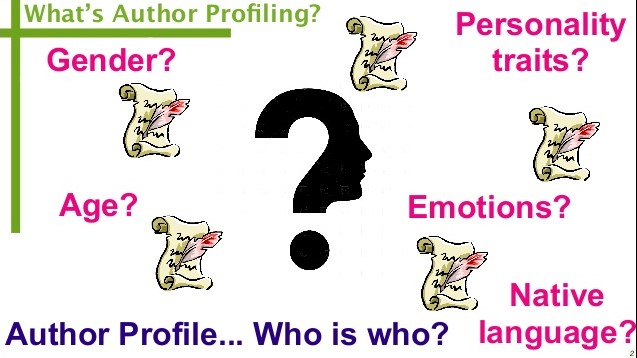
\includegraphics[scale=0.35]{author-profiling-task}}

\end{frame}


%------------------------------------------------




\begin{frame}
\frametitle{Our task}
\vspace{-2mm}
\begin{itemize}
	\item Predicting author profiling aspects
	\begin{itemize}
		\item Demographics (Classification)
		\begin{itemize}
			\item age
			\item gender
		\end{itemize}
		\item Big Five personality traits (Regression)
		\begin{itemize}
			\item extroversion
			\item stability
			\item agreeableness
			\item conscientiousness
			\item openness
		\end{itemize}
	\end{itemize}
\end{itemize}
\end{frame}



%------------------------------------------------

%------------------------------------------------
\section{Dataset}
%------------------------------------------------

%------------------------------------------------

\begin{frame}
\frametitle{Dataset}
\begin{itemize}
	\item English tweets dataset from PAN 2015 competition
	\begin{itemize}
			\item XML format, 152 users
			\item Age and gender labels
			\begin{itemize}
				\item 18-24, 25-34 34-49, 50+
				\item M, F
			\end{itemize}
			\item Personality traits
			\begin{itemize}
				\item normalized numeric rating in [-0.5,0.5] range
			\end{itemize}
		\end{itemize}
\end{itemize}
\end{frame}

%------------------------------------------------

%------------------------------------------------
\section{Preprocessing}
%------------------------------------------------

%------------------------------------------------

\begin{frame}
\frametitle{Preprocessing}
\begin{itemize}
	\item Creating a document of tweets for each user
	\item Cleaning tweets from
	\begin{itemize}
		\item XML tags
		\item hashtags
		\item @mentions
		\item URLs
		\item dupicates
	\end{itemize}
\end{itemize}
\end{frame}

%------------------------------------------------

\begin{frame}
\frametitle{Features}
\begin{itemize}
	\item Ovdje opisati što o featurima
\end{itemize}
\end{frame}


%------------------------------------------------
\section{Feature extraction}
%------------------------------------------------

%------------------------------------------------

\begin{frame}
\frametitle{Feature extraction}


\end{frame}

%------------------------------------------------
\section{Supervised learning model}
%------------------------------------------------

\begin{frame}
\centering
\frametitle{Models}

\end{frame}
%------------------------------------------------

\begin{frame}
\frametitle{Model selection}
\centerline{Odabri modela.}
\end{frame}

%------------------------------------------------
\section{Results}
%------------------------------------------------

\begin{frame}[fragile] % Need to use the fragile option when verbatim is used in the slide
\frametitle{Results}

\centerline{Rezultati.}
\end{frame}

%------------------------------------------------
\begin{frame}[fragile] % Need to use the fragile option when verbatim is used in the slide
\frametitle{Implementation}
\vspace{1cm}
\begin{itemize}
\setlength\itemsep{1em}
	\item Python Python
	\item Sklearn Sklearn

\end{itemize}


\end{frame}

%-----------------------------------------------

%------------------------------------------------

\begin{frame}
\frametitle{Conclusion}
\vspace{1.25cm}
\begin{itemize}
\setlength\itemsep{1em}
	\item Zaključak rada. 
\end{itemize}
\end{frame}

%------------------------------------------------

\begin{frame}
\vspace{1.25cm}
\frametitle{End}
\centerline{Thank you for attention.}
\vspace{0.5cm}
\centerline{Questions, comments ?}
\end{frame}

%----------------------------------------------------------------------------------------

\end{document} 